\section{Requests}
\label{sec:requests}

Use an Updated Lagrangian Formulation and four 4-node quadrilateral elements to simulate simple shear loading.
The bottom edge of the specimen is fixed in place while a constant velocity is applied to the top in the $\vec{x}$ direction.

\begin{figure}[h]
    \centering
    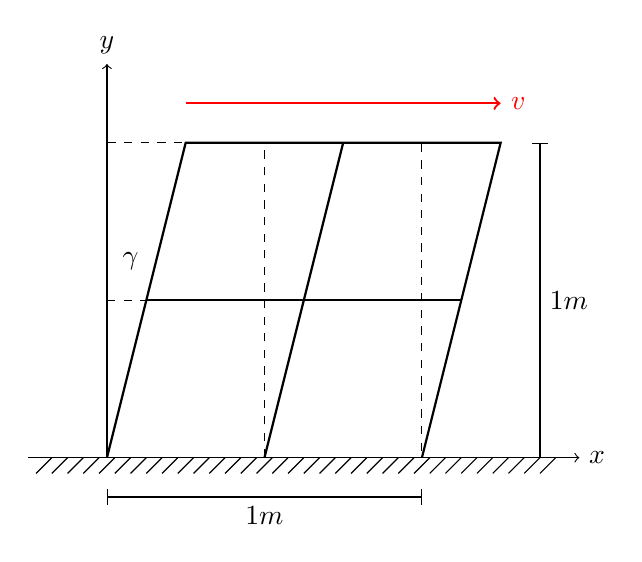
\begin{tikzpicture}

        \draw[->] (-1, 0) -- ++(7, 0) node[right]{$x$};
        \draw[->] (0, 0) -- ++(0, 5) node[above]{$y$};

        \draw[thick] (0, 0) -- ++(1, 4) -- ++(4, 0) -- ++(-1, -4);
        \draw[thick] (2, 0) -- ++(1, 4);
        \draw[thick] (0.5, 2) -- ++(4, 0);

        \draw[dashed] (0, 0) -- ++(0, 4) -- ++(4, 0) -- ++(-0, -4);
        \draw[dashed] (2, 0) -- ++(0, 4);
        \draw[dashed] (0, 2) -- ++(4, 0);

        \draw[|-|] (0, -0.5) -- ++(4, 0) node[midway, below]{$1m$};
        \draw[|-|] (5.5, 0) -- ++(0, 4) node[midway, right]{$1m$};

        \draw[->, thick, red] (1, 4.5) -- ++(4, 0) node[right]{$v$};

        \node at (0.3, 2.5) {$\gamma$};

        \foreach \x in {-0.7, -0.5, ..., 5.7}
        \draw (\x, 0) -- ++(-0.2, -0.2);

    \end{tikzpicture}
    \caption{Problem representation in its initial (dashed lines) and final (solid lines) configuration.}
    \label{fig:problem_representation}
\end{figure}

The material is made out of aluminum with density $\rho = 2700 \text{kg/m}^3$, Young's modulus $E = 70 \text{GPa}$, and Poisson's ratio $\nu = 0.3$.

Under the loading condition of $v = 1 \text{m/s}$ applied to the top three nodes:

\begin{itemize}
    \item Plot the average shear stress $\sigma_{12}$ as a function of shear strain until $\gamma = 0.07$.
          Use the \textbf{Truesdell objective rate} to update stress, $\boldsymbol{\sigma}^{oT} = \boldsymbol{C} : \boldsymbol{D}$.
    \item Plot the position of the nodes before and after loading the system.
    \item The loading speed, $v = 1 \text{m/s}$, was intentionally high for the sake of computation time.
          If the velocity is more realistic, such as $v = 0.001 \text{m/s}$, what can be done to further reduce the computation time?
\end{itemize}

\begin{table}[H]
    \centering
    \begin{tabular}{|c|c|c|}
        \hline
        \textbf{Parameter} & \textbf{Value} & \textbf{Unit}                    \\ \hline
        $E$                & $70$           & $\text{GPa}$                     \\ \hline
        $\nu$              & $0.3$          & $\text{-}$                       \\ \hline
        $\rho$             & $2700$         & $\text{kg/m\textsuperscript{3}}$ \\ \hline
        $L_x$              & $1$            & $\text{m}$                       \\ \hline
        $L_y$              & $1$            & $\text{m}$                       \\ \hline
    \end{tabular}
    \caption{Parameters of the plate element.}
    \label{tab:parameters_of_the_system}
\end{table}
